% Chapter 5

\chapter{Benchmark results and discussion} % Main chapter title
\label{Results} % For referencing the chapter elsewhere, use \ref{Chapter1} 

\lhead{Chapter \ref{Results}. \emph{Benchmark results and discussion}} % This is for the header on each page - perhaps a shortened title

Chapter \ref{CUDAHMMER3} described several approaches to optimize the cudaHmmsearch implementation. This chapter presents the performance measurements when experimenting with these approaches on a GPU and on a multi-core CPU.
%----------------------------------------------------------------------------------------

\section{Benchmarking environment}
\label{bench}
The benchmarking environment was set up in the Kronos 840S desktop workstation produced by Ciara Technologies Inc. \citep{Kronos} The Kronos has the following configuration:
 
\begin{itemize}
 \item CPU host : Intel Core i7-3960X with 6 cores, 3.3GHz clock speed, 64GB RAM
 \item GPU device : NVIDIA Quadro K4000 graphics card with 3 GB global memory, 768 Parallel-Processing Cores, 811 MHz GPU Clock rate, CUDA Compute Capability 3.0.
 \item Software system : The operating system used was Ubuntu 64 bit Linux v12.10; the CUDA toolkit used was version 5.5.
\end{itemize}

The data used in the experiments consisted of :

\begin{itemize}
 \item Target sequences database : Two target sequences databases was used in the benchmark experiments: \textbf{SP201309} and \textbf{N201404}. SP201309 was Swiss-Prot database in fasta format released in September 2013 \citep{UniProt} containing 540,958 sequences with length varying from 2 to 35,213 amino acids, comprising 192,206,270 amino acids in total, more than 258MB in file size. N201404 was much larger NCBI NR database in fasta format released in April 2014 \citep{NCBI} containing 38,442,706 sequences with length varying from 6 to 41,943 amino acids, comprising 13,679,143,700 amino acids in total, more than 24GB in file size.
 \item Query profile HMMs : We tested 5 profile HMMs of length 149, 255, 414, 708 and 1111 states respectively, detailed in Table \ref{tab.phmms}. The globins4 with a length of 149 states was distributed with the HMMER source \citep{Hsource}. The other 4 HMMs were taken directly from the Pfam database \citep{Pfam}.\\
 \begin{table}[H]
 \centering
 \begin{tabular}{|c|c|c|c|c|c|}\hline
 \textbf{Name} & globins4 & 120\_Rick\_ant & 2HCT & ACC\_central & AAA\_27 \\\hline
 \textbf{Accession number} & - & PF12574.3 & PF03390.10 & PF08326.7 & PF13514.1 \\\hline
 Length & 149 & 255 & 414 & 708 & 1111 \\\hline
 \end{tabular}
 \caption{\fontfamily{pag}\selectfont Profile HMMs used in benchmarking. \label{tab.phmms} The globins4 has no Accession number.}
 \end{table}
\end{itemize}

The measurement of performance that was used was GCUPS (Giga Cell Units Per Second) which was determined as follows:

\begin{itemize}
 \item Measuring method\\ 
 \begin{equation*}
   GCUPS = \frac{L_q * L_t}{T * 1.0e09}
 \end{equation*}
 where $L_q$ is the length of query profile HMM, i.e. the number of the HMM states, $L_t$ is the total residues of target sequences in the database, $T$ is the execution time in second.\\ 
 The execution time of the application was timed using the C clock() instruction.\\
 All programs were compiled using GNU g++ with the -O3 option and executed independently in a 100\% idle system.
\end{itemize}

%----------------------------------------------------------------------------------------

\section{Performance Results}
We did four experiments for our implementation cudaHmmsearch benchmarking. Each experiment was done in the same benchmarking environment as described in Section \ref{bench}. This section will explain each experiment and show the results and the related analysis of these experiments.

\subsection{Comparison with less optimized approaches}

\paragraph*{Experiment A : }This experiment tested the performance of cudaHmmsearch with several selected approaches. To show the performance impact of the selected optimization approaches, the performance of the corresponding implementation was benchmarked and the corresponding improvement was measured in percentage compared with that of previous approach.
All tests were taken searching the globins4 profile HMM against the SP201309 database.

\begin{table}[H]
\centering
\begin{tabular}{|c|c|c|c|}\hline
\shortstack{\textbf{Description of} \\ \textbf{approach}} & \shortstack{\textbf{Execution} \\ \textbf{time (s)}} & \shortstack{\textbf{Performance}\\ (GCUPS)} & \shortstack{\textbf{Improvement}\\ \textbf{(\%)}}\\\hline
Initial implementation & 227.178 & 0.126 & - \\\hline
SIMD Video Instruction & 125.482 & 0.228 & 81 \\\hline
\shortstack{Minimizing global\\memory access} & 16.449 & 1.741 & 664 \\\hline
\shortstack{Async memcpy \&\\Multi streams} & 9.463 & 3.026 & 74 \\\hline
\shortstack{Coalescing of\\global memory} & 6.565 & 4.362 & 44 \\\hline
Texture memory & 5.370 & 5.333 & 22 \\\hline
Sorting Database & 2.346 & 12.207 & 129 \\\hline
Distributing workload & 1.650 & 17.357 & 42 \\\hline
\end{tabular}
\caption{\fontfamily{pag}\selectfont \textbf{Performance of optimization approaches.} The table shows the result of Experiment A, using cudaHmmsearch to search the globins4 profile HMM against the SP201309 database. The fourth column \textbf{Improvement} is measured in percentage compared with the previous approach. The row `Coalescing of global memory' is benchmarked only for the $dp$ matrix. The row `Texture memory' is benchmarked only for the query profile texOMrbv 2D texture. \label{tab.opt}}
\end{table}

Table \ref{tab.opt} shows the testing results of ExperimentA. The fourth column `Improvement' is measured in percentage compared with the previous approach. `Initial implementation' described in Section \ref{Aimpl} is used as the baseline. `SIMD Video Instruction' is the approach described in Section \ref{video}. `Minimizing global memory access' is the approach of reducing the frequency of global memory access described in Section \ref{Afre}. `Async memcpy \& Multi streams' is the approach described in Section \ref{asyn}. `Coalescing of global memory' is the approach of coalescing access described in Section \ref{coal}. `Texture memory' is the approach described in Section \ref{tex}. `Sorting Database' is the approach described in Section \ref{dbsort}. `Distributing workload' is the approach described in Section \ref{workload}.

The graphic view corresponding to the above table is shown in Figure \ref{fig:imp}. 

\begin{figure}[!htb]
	\centering
	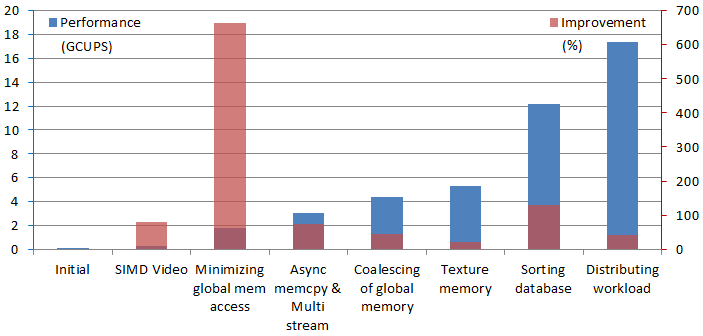
\includegraphics[totalheight=0.28\textheight]{Figures/improve.png}
	\caption{\fontfamily{pag}\selectfont \textbf{Performance of optimization approaches.} The data of this chart come from Table \ref{tab.opt} for Experiment A. The blue bar is Performance (in GCUPS) of each approach, corresponding to the left Y axis. The red bar is Improvement in \% corresponding to the right Y axis.}
	\label{fig:imp}
\end{figure}

From Figure \ref{fig:imp}, it can be seen that the global memory optimizations are the most important area for performance. Several factors are related to global memory accesses, including the highest 663\% minimizing global memory access, coalescing of global memory and texture memory. To make all threads in a warp execute similar tasks, the auxiliary sorting database also plays an important role in optimizations.

\subsection{Practical benchmark}
\label{Pbench}
\paragraph*{Experiment B : }This experiment tested the real-world performance of the final cudaHmmsearch implementation, with the optimizations discussed in Chapter \ref{CUDAHMMER3}. 
This was done by using the fully optimized cudaHmmsearch to search the much large N201404 database for the 5 profile HMMs in Table \ref{tab.phmms}. As comparison, the same searches were executed by hmmsearch of HMMER3 on one CPU core on the Kronos machine. The result of Experiment B is shown in Table \ref{tab.pb}.

The results of the benchmarks are shown in graphical form in Figure \ref{fig:len}. The GPU cudaHmmsearch performance hovers just above 25 GCUPS, while the CPU hmmsearch only around 10 GCUPS. The whole performance of cudaHmmsearch is stable with various lengths of query HMMs. On average, cudaHmmsearch has a speedup of 2.53x over hmmsearch of HMMER3. 

Figure \ref{fig:len} also shows that the performance of both GPU and CPU searching for AAA\_27 dropped significantly compared with other searches. The reason can be seen from Table \ref{tab.sta} listing the internal pipeline statistics summary for searching globins4 and AAA\_27. Table \ref{tab.sta} shows the total number of target sequences in the N201404 database and the number of passed sequences after each filter. After every filter, the number of passed sequences for searching AAA\_27 with 1111 states is much more than that of globins4 with 149 states. This means that for searching AAA\_27, more target sequences are processed than globins4 in each filter after the MSV filter. At the same time, each of these filters is more time-consuming than the MSV filter. This results in the AAA\_27 performance dropping significantly.

\begin{table}[H]
\centering
\begin{tabular}{|c|c|c|c|c|c|}\hline
\shortstack{\textbf{Profile HMM} \\ \textbf{(length)}} & \multicolumn{2}{|c|}{\shortstack{\textbf{hmmsearch} \\ (s) (GCUPS)}} & \multicolumn{2}{|c|}{\shortstack{\textbf{cudaHmmsearch} \\ (s) (GCUPS)}} & \shortstack{\textbf{Speedup} \\ (times)} \\\hline
\shortstack{globins4 \\ (149)} & 217.54s & 9.37GCUPS & 88.63s & 23.00GCUPS & 2.45 \\\hline
\shortstack{120\_Rick\_ant \\ (255)} & 297.52s & 11.72GCUPS & 108.42s & 32.17GCUPS & 2.74 \\\hline
\shortstack{2HCT \\ (414)} & 484.68s & 11.68GCUPS & 188.72s & 30.01GCUPS & 2.57 \\\hline
\shortstack{ACC\_central \\ (708)} & 809.97s & 11.96GCUPS & 295.02s & 32.83GCUPS & 2.75 \\\hline
\shortstack{AAA\_27 \\ (1111)} & 2203.36s & 6.90GCUPS & 1034.96s & 14.68GCUPS & 2.13 \\\hline
\textbf{Average} & \multicolumn{2}{|c|}{-} & \multicolumn{2}{|c|}{-} & 2.53 \\\hline
\end{tabular}
\caption{\fontfamily{pag}\selectfont \textbf{Result of Practical benchmark.} \label{tab.pb} The table shows the result of Experiment B, using the fully optimized cudaHmmsearch and hmmsearch of HMMER3 to search the 5 profile HMMs against the N201404 database. In the column of hmmsearch and cudaHmmsearch, the left sub-column is execution time in second and the right sub-column is performance in GCUPS. Speedup is measured in times of cudaHmmsearch performance over that of hmmsearch.}
\end{table}

\begin{figure}[!htb]
	\centering
	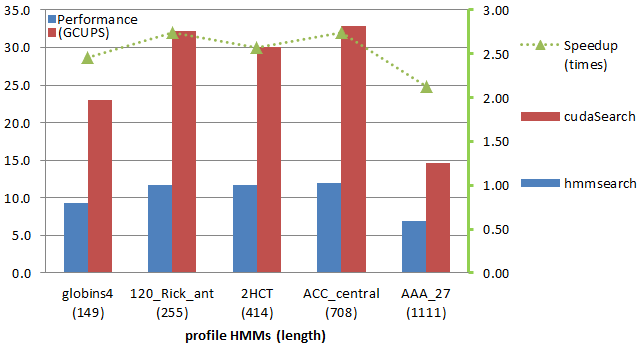
\includegraphics[totalheight=0.36\textheight]{Figures/lengths.png}
	\caption{\fontfamily{pag}\selectfont \textbf{Practical benchmarks.} The data of this chart come from Table \ref{tab.pb}. The blue and red bar is Performance (in GCUPS) of hmmsearch and cudaHmmsearch respectively, corresponding to the left Y axis. The green dot line is Speedup (in times) of cudaHmmsearch performance over that of hmmsearch, corresponding to the right Y axis.}
	\label{fig:len}
\end{figure}

\begin{table}[H]
\centering
\begin{tabular}{|c|c|c|}\hline
\shortstack{\textbf{Query profile HMM(length)}} & \shortstack{\textbf{globins4 (149 states)}} & \shortstack{\textbf{AAA\_27 (1111 states)}}\\\hline
Target sequences & 38,442,706 & 38,442,706 \\\hline
Passed MSV filter & 1,195,043 & 4,305,846 \\\hline
Passed bias filter & 973,354 & 1,671,084 \\\hline
Passed Viterbi filter & 70,564 & 322,206 \\\hline
Passed Forward filter & 7,145 & 17,719 \\\hline
\end{tabular}
\caption{\fontfamily{pag}\selectfont \textbf{Internal pipeline statistics summary.}\label{tab.sta} The table shows the total number of target sequences in the N201404 database and the number of passed sequences after each filter for searching globins4 and AAA\_27 in the Experiment B.}
\end{table}

\subsection{Comparison with multicore CPU}
\paragraph*{Experiment C : } This experiment tested the performance of cudaHmmsearch and hmmsearch of HMMER3 running with multiple CPU cores. The Kronos experiment system has an Intel Core i7-3960X CPU with six cores.

A benchmark to study the impact of multiple CPU cores has not been used in the articles cited in this thesis. The purpose of Experiment C is to show how the performance increase or decrease with the use of more CPU cores.

The experiment was done by executing the fully optimized cudaHmmsearch and hmmsearch of HMMER3 with one to six CPU cores, searching the N201404 database for the 120\_Rick\_ant profile HMM. The result of Experiment C is shown in Table \ref{tab.mcpu}.

\begin{table}[H]
\centering
\begin{tabular}{|c|c|c|c|c|c|c|}\hline
\shortstack{\textbf{Performance} \\ \textbf{(GCUPS)}} & \shortstack{1 CPU \\ core} & \shortstack{2 CPU \\ cores} & \shortstack{3 CPU \\ cores} & \shortstack{4 CPU \\ cores} & \shortstack{5 CPU \\ cores} & \shortstack{6 CPU \\ cores} \\\hline
cudaHmmsearch & 32.17 & 50.22 & 57.70 & 59.14 & 59.39 & 59.29 \\\hline
hmmsearch & 11.72 & 23.28 & 29.22 & 44.15 & 46.19 & 44.69 \\\hline
Speedup (times) & 2.74 & 2.16 & 1.97 & 1.34 & 1.29 & 1.33 \\\hline
\end{tabular}
\caption{\fontfamily{pag}\selectfont \textbf{Result of Comparison with multicore CPU.} \label{tab.mcpu} The table shows the result of Experiment C, using the fully optimized cudaHmmsearch and hmmsearch of HMMER3 to search the 120\_Rick\_ant profile HMM against the N201404 database with one to six CPU cores involved in computing. }
\end{table}

The graphic view of the benchmark is shown in Figure \ref{fig:cpuCores}. The number above each bar is the Performance in GCUPS. As can be seen, from 1 CPU core to 4 CPU cores, both cudaHmmsearch performance and hmmsearch performance increase almost linearly. From then on, perhaps due to complex scheduling among CPU cores and only one I/O to load sequences from the database for CPU cores, the extra CPU cores do not contribute much to either cudaHmmsearch or hmmsearch execution. Even worse, six CPU cores have a negative effect compared to five CPU cores.

\begin{figure}[!htb]
	\centering
	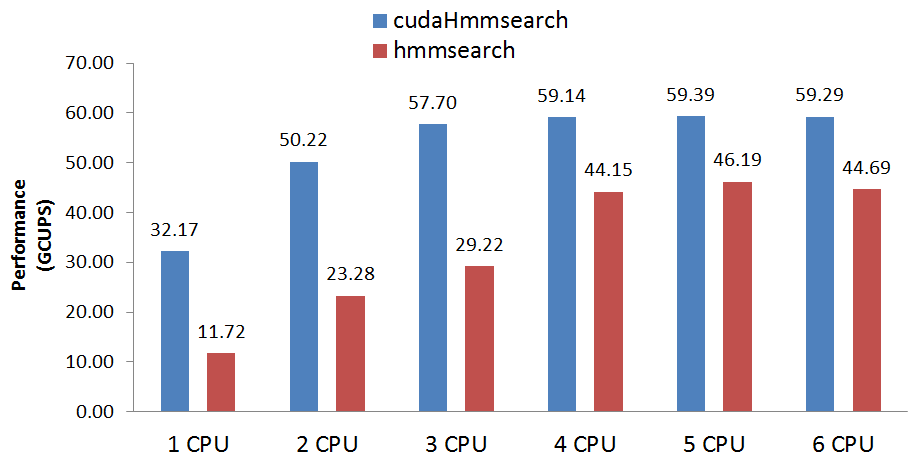
\includegraphics[totalheight=0.25\textheight]{Figures/cpuCores.png}
	\caption{\fontfamily{pag}\selectfont \textbf{Comparison with multicore CPU.} The data of this chart come from Table \ref{tab.mcpu} for Experiment C. The number above each bar is the Performance in GCUPS.}
	\label{fig:cpuCores}
\end{figure}

\subsection{Comparison with other implementations}
\paragraph*{Experiment D : } This experiment tested the performance of cudaHmmsearch with previous hmmsearch solutions: HMMER2.3.2 \citep{HMMER2}, GPU-HMMER2.3.2 \citep{GPUHMM} and HMMER3 \citep{Hsource}.
All tests were taken using the fully optimized cudaHmmsearch and the hmmsearch in HMMER2.3.2, GPU-HMMER2.3.2 and HMMER3 to search against the SP201309 database for the globins4 profile HMM. The hmmsearch in HMMER2.3.2 and HMMER3 were executed on one CPU core. The hmmsearch in GPU-HMMER2.3.2 was executed on one GPU using one CPU core. The result of Experiment D is shown in Table \ref{tab.hmms}.

\begin{table}[H]
\centering
\begin{tabular}{|c|c|c|c|c|}\hline
\shortstack{Application \\ (Device)} & \shortstack{HMMER2.3.2 \\ (CPU)} & \shortstack{GPU-HMMER2.3.2 \\ (GPU)} & \shortstack{HMMER3 \\ (CPU)} & \shortstack{cudaHmmsearch \\ (GPU)} \\\hline
\shortstack{Performance\\ (GCUPS)} & 0.14 & 0.95 & 8.47 & 17.36 \\\hline
Speedup (times) & 1.00 & 6.79 & 60.50 & 124.00 \\\hline
\end{tabular}
\caption{\fontfamily{pag}\selectfont \textbf{Result of Comparison with other implementations.} \label{tab.hmms} The table shows the result of Experiment D, searching against the SP201309 database for the globins4 profile HMM. The hmmsearch in HMMER2.3.2 and HMMER3 were executed on one CPU core. The hmmsearch in GPU-HMMER2.3.2 and the fully optimized cudaHmmsearch was executed on one GPU using one CPU core. Speedup uses the performance of HMMER2.3.2 as baseline 1.00 and is measured in times of each performance over that of HMMER2.3.2.}
\end{table}

As seen from the Figure \ref{fig:hmms}, since the release of HMMER2.3.2 in Oct 2003, accelerating hmmsearch researches on both CPU and GPU have achieved significant improvement.

\begin{figure}[!htb]
	\centering
	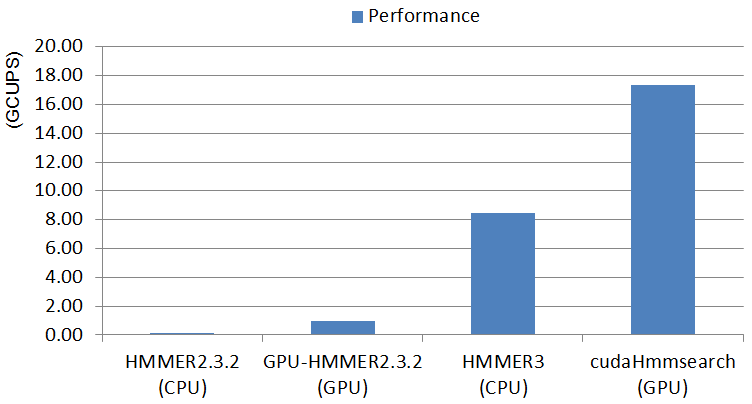
\includegraphics[totalheight=0.28\textheight]{Figures/manyhmms.png}
	\caption{\fontfamily{pag}\selectfont \textbf{Comparison with other implementations}. The data of this chart come from Table \ref{tab.hmms} for Experiment D.}
	\label{fig:hmms}
\end{figure}

%----------------------------------------------------------------------------------------

% Chapter 6

\chapter{Conclusions} % Main chapter title

\label{Conclusions} % For referencing the chapter elsewhere, use \ref{Chapter1} 

\lhead{Chapter \ref{Conclusions}. \emph{Conclusions}} % This is for the header on each page - perhaps a shortened title

A fully-featured and accelerated HMMER3 protein search tool \emph{cudaHmmsearch} was implemented on CUDA-enabled GPU. It can search the protein sequence database for profile HMMs.

%----------------------------------------------------------------------------------------

\section{Summary of Work}
Our research work started with dynamic programming, the common characteristic of Swith-Waterman algorithm, Viterbi algorithm and MSV algorithm, which are famous protein sequence alignment algorithms in Bioinformatics.
We summarized the technologies of accelerating Swith-Waterman algorithm on a CUDA-enabled GPU, which has been widely researched. We also briefly presented GPU acceleration work related to Viterbi algorithm.

After analyzing the core application \emph{hmmsearch} in HMMER3, we found the key hotspot MSV filter for accelerating hmmsearch. We presented the details of our \emph{cudaHmmsearch} implementation and optimization approaches. At the same time, we also discussed and analyzed the advantages and limitations of GPU hardware for CUDA parallel programming. Then we summarized six steps for better performance of CUDA programming: 1)assessing the application; 2)profiling the application; 3)optimizing memory usage; 4)optimizing instruction usage; 5)maximizing parallel execution; 6)considering the existing libraries.

We performed comprehensive benchmarks. The results were analyzed and the efficiency of the \emph{cudaHmmsearch} implementations on the GPUs was demonstrated. We achieved 2.5x speedup over the single-threaded HMMER3 CPU SSE2 implementation. The performance analysis showed that GPUs are able to deal with intensive computations, but are very sensitive to random accesses to the global memory.

The solutions in this thesis were designed and customized for current GPUs, but we believe that the principles studied here will also apply to future many-core GPU processors, provided the GPU is CUDA-enabled. Here is the complete list of CUDA-enabled GPUs: \url{https://developer.nvidia.com/cuda-gpus}.

%----------------------------------------------------------------------------------------

\section{Limitations of Work}
There are some weak points in our work summarized as follows:

Although our \emph{cudaHmmsearch} can search against an unsorted protein sequence database, it gains 129\% improvement by searching against a sorted database according to benchmark Table \ref{tab.opt}. Although the program for sorting database is provided, the user may be unaware of this and run \emph{cudaHmmsearch} against an unsorted database. It is better for the program to evaluate the database automatically and prompt the user to sort if necessary.

We use a block reading method to process very large databases. However, the number of sequences for each block reading is fixed. Hence the number of threads launched in GPU kernel is also fixed. For those sequences with shorter lengths, it is better to use dynamic block reading to load more sequences, so as to increase the occupancy of GPU threads and achieve better performance.

%----------------------------------------------------------------------------------------

\section{Recommendations for Future Research}
The limitations noted in the last section call attention to several areas that we deem worthy of further improvement and investigation. The suggested topics are placed under the following headings.

\subsection*{Forward filter for no threshold}
By default, the top-scoring of target sequences are expected to pass each filter. Alternatively, the -\emph{-max} option is available for those who want to make a search more sensitive to get maximum expected accuracy alignment. The option causes all filters except the Forward/Backward algorithm to be bypassed. According to practical benchmarking in Section \ref{Pbench}, the performance decreased greatly due to much more calculation in the Forward algorithm. So our next research should be focused on accelerating the Forward algorithm on a CUDA-enabled GPU.

\subsection*{Multiple GPUs approach}
Since currently we have no multiple GPUs within a single workstation, we did not research on multiple GPUs approach. However, CUDA already provides specific facilities for multi-GPU programming, including threading models, peer-to-peer, dynamic parallelism and inter-GPU synchronization, etc. Almost all PCs support at least two PCI-E slots, allowing at least two GPU cards to insert almost any PC. Looking forward, we should also investigate multi-GPU solutions.

%----------------------------------------------------------------------------------------
